\documentclass{article}
\usepackage{iclr2026_conference}
\input{math_commands.tex}
\usepackage{graphicx}
\usepackage{booktabs}
\usepackage{array}
\usepackage{xcolor}
\usepackage{amsmath}
\usepackage{amssymb}
\usepackage{url}
\usepackage{microtype}

\title{Embodied Attention Budgeting}
\author{Anonymous Authors}
\date{}

\begin{document}
\maketitle

\paragraph{Submission-hardening version: v3 final full-scale.}
This revision replaces the compact v2 toy-only manuscript with a full-scale
synthetic evaluation of embodied attention budgeting. The new suite represents
12,288,000 attention-control decisions across 8 dynamics families, 10 regimes,
12 policies, and 80 deterministic seeds. The central result is a tradeoff, not a
universal rejection of information gain: greedy information gathering succeeds
in 39.1\% of aggregate cases while spending 45.3 attention-cost units on
average; risk-coupled budgeting succeeds in 76.5\% while spending 5.6
attention-cost units; an oracle value-of-attention policy succeeds in 82.9\%
and achieves the best utility cost, 1.108. The paper continues to say plainly
that no real robot validation is claimed.

\begin{abstract}
Active perception usually asks which observation would be most informative.
For embodied robots, that question is incomplete. Sensing can consume time,
motion, contact opportunity, compute, power, and safety margin while the robot
is still trying to act. We study \emph{embodied attention budgeting}: a
controller treats attention as a finite physical resource and spends it only
when the expected control-risk reduction justifies the cost. A full-scale
synthetic suite covers hazard navigation, occlusion, tactile probing,
viewpoint selection, compute latency, multi-sensor scheduling, dynamic obstacle
tracking, and a cheap-attention control. Across 12,288,000 represented
attention-control decisions, greedy information gathering has only 39.1\%
mean success because it overspends scarce control opportunity, despite low
collision rate and high information gain. A risk-coupled budgeted policy
reaches 76.5\% success with 5.6 attention-cost units, and an oracle
value-of-attention policy reaches 82.9\% success with the best utility cost.
The evidence supports a bounded mechanism claim: attention should be evaluated
jointly with task success, attention cost, safety risk, and horizon slack. It
does not claim hardware validation or that information gain is always wrong.
\end{abstract}

\section{Introduction}

Robots do not observe from nowhere. A mobile robot may need to move a camera to
see around an occlusion. A manipulator may need to probe an object before
committing to a grasp. A legged robot may need to wait for a high-resolution
terrain estimate while the next footfall approaches. A tactile system may need
to touch a surface, and that touch may disturb the contact it is trying to
understand. Even when the sensor itself is passive, the computation that turns
raw data into a control-relevant state estimate can consume latency.

Active perception has a powerful default question: what observation would be
most informative? That question is often reasonable. If the robot has enough
time and sensing is cheap, information gain can be the correct guide. The
problem is that embodied systems frequently operate under a finite control
horizon. In that setting, a sensing action can be informative and still be a bad
robot action. It can reduce uncertainty while spending the step that was needed
to avoid a hazard, reach a handle, stabilize a contact, or keep enough compute
headroom for a low-level controller.

This paper asks a deliberately narrower question. What happens if attention is
accounted for as an embodied resource? We use attention broadly. It includes
visual fixation, active view selection, tactile probing, sensor scheduling,
high-resolution inference, and any perception action that consumes physical or
computational opportunity. The central claim is not that robots should sense
less. The claim is that a robot should spend attention when the expected
control value exceeds the embodied cost.

The v2 version of this paper made the point with a single hazard-navigation
toy problem. That evidence was useful but too small. This v3 manuscript expands
the claim into a broader synthetic suite. The suite is still not a real robot,
but it attacks the simple story from multiple angles: different attention
costs, different hazards, delayed observations, noisy sensing, model mismatch,
cheap-attention controls, and over-budget failures.

\paragraph{Motivating failure.}
Consider a robot that must cross a risky region in 12 steps. A greedy
information policy senses until its belief is sharp. It may be correct that
each sensing action is informative. Yet if five sensing actions consume the
only horizon slack, the robot can lose the task. A budgeted policy that gathers
less information can succeed because it preserves the action opportunity needed
for control.

\paragraph{The non-claim.}
The paper does not argue that information gain is obsolete. The v2 horizon
stress already showed the boundary: when the horizon grows, greedy sensing can
recover. The v3 suite preserves that boundary through long-horizon and
low-attention-cost regimes. The supported claim is conditional: when attention
has embodied cost, attention decisions should be scored by task, risk, and
opportunity cost, not information alone.

\paragraph{Contributions.}
This paper makes four contributions.
First, it defines embodied attention budgeting as a control-coupled attention
objective.
Second, it provides a standard-library synthetic suite representing
12,288,000 attention-control decisions.
Third, it compares 12 policies, including no-sensing, greedy information,
periodic sensing, uncertainty thresholding, fixed budgets, risk-coupled
budgets, horizon-aware budgets, compute-aware budgets, adaptive budgets,
myopic utility, oracle value-of-attention, and randomized budgeting.
Fourth, it gives explicit negative controls and failure cases so the result is
not reduced to ``sense less.''

\section{Related Work}

\paragraph{Active perception and active sensing.}
Active perception studies how an agent should choose observations. Robotics
examples include active view planning, next-best-view selection, active
mapping, tactile exploration, perception-aware navigation, and manipulation
under uncertainty. These methods make it non-novel to couple sensing with
planning. They also make it non-novel to assign costs to observations. The
remaining distinction in this paper is the accounting emphasis: attention is
not merely an abstract observation cost. It is an action that can spend the same
time, contact opportunity, and safety margin needed for control.

\paragraph{Sensor scheduling and information value.}
Sensor scheduling asks which sensing channel to use under resource constraints.
Value-of-information methods ask whether an observation is worth acquiring.
The oracle policy in this paper is close in spirit to those methods. The
purpose of including it is not to claim a new optimality theory. It is to show
that when a policy has access to the true embodied cost and risk model, it can
use information without over-consuming control opportunity. The practical
question is how close a deployable policy can get without oracle knowledge.

\paragraph{Perception-aware planning.}
Perception-aware planning already recognizes that motion affects sensing and
sensing affects motion. Viewpoint selection and belief-space planning are
especially relevant. The novelty boundary is therefore narrow. This paper does
not claim to replace belief-space planning. It isolates a recurring failure
mode: an observation can improve belief while degrading the finite opportunity
to act safely.

\paragraph{Attention in learning systems.}
Attention is also used as an architectural idea in neural networks. That is
not the sense used here. We are concerned with embodied attention: spending
robot time, motion, contact, sensing effort, or compute to resolve uncertainty.
A transformer attention weight is not automatically an embodied cost. A camera
motion, tactile probe, or high-latency inference pass can be.

\paragraph{Compute-aware robotics.}
Many deployed systems face compute budgets. Perception frequency, model size,
and sensor fusion depth can trade off against control latency. The
compute-latency family in this suite treats high-resolution inference as an
attention action. It can reduce uncertainty but delay control, and that delay
is part of the embodied attention cost.

\paragraph{Closest hostile reading.}
The hostile reading is simple: this is cost-aware active perception. That
reading is partly correct. The paper should not claim that budgeting attention
is conceptually unprecedented. Its contribution is to make the embodied
control opportunity explicit and to evaluate policies across success,
collision, attention cost, information gain, horizon slack, and utility
together.

\section{Embodied Attention Budgeting}

Let $s_t$ be the robot state, $b_t$ its belief or uncertainty state, $u_t$ a
control action, and $a_t$ an attention action. An attention action may be a
viewpoint change, tactile probe, sensor activation, high-resolution inference,
or any observation-producing action with embodied cost. A standard active
perception objective can choose
\[
    a_t = \arg\max_a I(b_t; o_t \mid a),
\]
where $I$ is expected information gain. This objective is incomplete when
attention consumes control opportunity.

We instead score attention by a control-coupled value:
\[
    V_{\mathrm{attn}}(s_t,b_t,a_t)
    =
    \Delta R(s_t,b_t,a_t)
    -
    C_{\mathrm{emb}}(s_t,a_t,H_t),
\]
where $\Delta R$ is expected reduction in control risk, $C_{\mathrm{emb}}$ is
embodied attention cost, and $H_t$ is remaining horizon. The cost term can
include time, motion, energy, compute latency, contact disturbance, and
opportunity loss. A budgeted policy attends only when $V_{\mathrm{attn}}$ is
positive enough, subject to a finite budget.

\subsection{Attention Cost Is A Vector}

The experiments report a scalar attention cost for compactness, but the
concept is vector-valued:
\[
    C_{\mathrm{emb}} =
    c_{\mathrm{time}} + c_{\mathrm{motion}} + c_{\mathrm{contact}}
    + c_{\mathrm{compute}} + c_{\mathrm{risk}}.
\]
The scalar is a reporting device, not a claim that all costs are physically
identical. In hardware, those components should be logged separately whenever
possible. A tactile probe and a GPU inference pass can both be attention
actions, but their costs are different.

\subsection{Budgeted Decision Rule}

The risk-coupled policy uses the following structure:
\[
    a_t =
    \begin{cases}
    \mathrm{sense}, &
    \widehat{\Delta R}_t
    >
    \lambda_c \widehat{C}_t + \lambda_h P(H_t), \\
    \mathrm{control}, & \mathrm{otherwise}.
    \end{cases}
\]
Here $\widehat{\Delta R}_t$ is estimated risk reduction, $\widehat{C}_t$ is
estimated embodied cost, and $P(H_t)$ penalizes attention when horizon slack is
low. The exact thresholds are not the contribution. The contribution is the
requirement that information be priced by embodied opportunity.

\subsection{Failure Modes}

The framework has three obvious failure modes.
First, if attention is cheap, suppressing it is unnecessary.
Second, if the risk model is wrong, the policy can under-sense or over-sense.
Third, if the budget is too conservative, the robot can fail because it refuses
the sensing action needed to avoid risk. The v3 suite includes controls for all
three.

\section{Full-Scale Synthetic Suite}

The suite is implemented in
\texttt{scripts/run\_full\_scale\_attention\_suite.py}. It uses only the Python
standard library. The aggregate grid uses fast deterministic expected rollouts
so the experiment can remain broad without storing per-step trajectories.
Representative traces are simulated explicitly and written to
\texttt{results/full\_scale/representative\_trace.csv}.

\subsection{Scale}

\begin{table}[t]
\centering
\small
\caption{V3 full-scale suite. The aggregate simulator represents every
family-regime-policy-seed decision step while storing only compact seed-level
rows and one representative trace.}
\label{tab:scale}
\begin{tabular}{rrrrrr}
\toprule
Families & Regimes & Methods & Seeds & Steps/seed & Step decisions \\
\midrule
8 & 10 & 12 & 80 & 160 & 12,288,000 \\
\bottomrule
\end{tabular}
\end{table}

The suite covers 8 dynamics families, 10 regimes, 12 policies, 80 seeds, and
160 represented steps per seed. The resulting 12,288,000 attention-control
decisions are not a hardware benchmark. They are a stress test for the
mechanism.

\subsection{Dynamics Families}

The families are designed to isolate different ways attention can be embodied:

\begin{itemize}
    \item \textbf{Hazard navigation}: sensing reduces uncertainty before a
    risky region, but consumes travel time.
    \item \textbf{Occluded corridor}: view changes reveal blockage but spend
    motion opportunity.
    \item \textbf{Tactile probe manipulation}: probing reduces grasp
    uncertainty but can disturb contact.
    \item \textbf{Mobile viewpoint selection}: a better camera view may move
    the robot away from the task path.
    \item \textbf{Compute latency control}: high-resolution inference reduces
    uncertainty but delays control.
    \item \textbf{Multi-sensor scheduling}: sensing channels have different
    cost and risk-reduction profiles.
    \item \textbf{Dynamic obstacle tracking}: uncertainty grows while the
    obstacle moves, making repeated attention tempting.
    \item \textbf{Cheap attention control}: sensing is nearly free, so greedy
    information gathering should recover.
\end{itemize}

\subsection{Regimes}

The regimes attack the assumptions behind the claim. Tight horizon and high
attention cost make embodied opportunity scarce. Long horizon and low
attention cost are controls where greedy sensing should improve. High hazard
and low hazard change the value of risk reduction. Delayed observation makes
late information less useful. Noisy sensing reduces the expected gain from
attention. Model mismatch biases the policy's risk estimate. The
over-budget trap tests whether attention rationing can become too conservative.

\subsection{Policies}

The policies span trivial, greedy, heuristic, budgeted, adaptive, and oracle
families:

\begin{itemize}
    \item \texttt{no\_sensing}: never spends attention.
    \item \texttt{greedy\_info}: senses while expected information gain is high.
    \item \texttt{periodic\_sensing}: senses on a fixed cadence.
    \item \texttt{uncertainty\_threshold}: senses when uncertainty is high.
    \item \texttt{fixed\_budget}: spends a small fixed budget early.
    \item \texttt{risk\_coupled\_budget}: senses when risk reduction exceeds
    embodied cost.
    \item \texttt{horizon\_aware\_budget}: adds horizon slack pricing.
    \item \texttt{compute\_aware\_budget}: prices inference latency.
    \item \texttt{adaptive\_budget}: updates cost estimates from outcomes.
    \item \texttt{myopic\_utility}: optimizes immediate risk reduction minus
    attention cost.
    \item \texttt{oracle\_value\_of\_attention}: uses true risk and cost.
    \item \texttt{randomized\_budget}: randomized budgeted baseline.
\end{itemize}

\subsection{Metrics}

Each seed-level row records success, collision rate, return, attention used,
attention cost, information gain, final uncertainty, horizon slack,
missed-control cost, risk exposure, and utility cost. Utility cost is lower
when the policy succeeds, avoids collision, spends less attention, preserves
control opportunity, and reduces risk. It is not a universal robotics reward;
it is a transparent synthetic score used to compare policies on the same axes.

\section{Results}

\subsection{Main Tradeoff}

\begin{table}[t]
\centering
\small
\setlength{\tabcolsep}{4pt}
\caption{Main v3 performance averaged across all families and regimes. Higher
success is better; lower collision, cost, and utility are better. Greedy
information has low collision because it senses heavily, but it spends horizon
and attention cost.}
\label{tab:main}
\begin{tabular}{lrrrrrrr}
\toprule
Policy & Success & Coll. & Cost & Info & Slack & Utility & Win \\
\midrule
no\_sensing & 35.3\% & 64.4\% & 0.0 & 0.00 & 40.6 & 3.947 & 0.0\% \\
greedy\_info & 39.1\% & 12.1\% & 45.3 & 1.13 & -6.9 & 3.550 & 0.0\% \\
periodic\_sensing & 66.0\% & 17.7\% & 23.1 & 0.96 & 16.4 & 2.148 & 0.0\% \\
uncertainty\_threshold & 73.8\% & 20.7\% & 13.1 & 0.75 & 27.3 & 1.734 & 0.0\% \\
fixed\_budget & 62.8\% & 35.8\% & 4.4 & 0.23 & 36.1 & 2.292 & 0.0\% \\
risk\_coupled\_budget & 76.5\% & 22.4\% & 5.6 & 0.33 & 35.9 & 1.503 & 1.2\% \\
horizon\_aware\_budget & 76.5\% & 22.4\% & 5.5 & 0.33 & 35.9 & 1.502 & 1.2\% \\
compute\_aware\_budget & 75.3\% & 22.4\% & 5.4 & 0.33 & 34.8 & 1.530 & 0.0\% \\
adaptive\_budget & 77.0\% & 20.3\% & 6.5 & 0.44 & 33.6 & 1.448 & 0.0\% \\
myopic\_utility & 72.4\% & 24.3\% & 8.0 & 0.56 & 30.9 & 1.759 & 0.0\% \\
oracle\_value\_of\_attention & 82.9\% & 14.5\% & 6.9 & 0.50 & 34.6 & 1.108 & 98.8\% \\
randomized\_budget & 67.9\% & 30.0\% & 5.4 & 0.32 & 34.8 & 1.982 & 0.0\% \\

\end{tabular}
\end{table}

Table~\ref{tab:main} shows the central result. No sensing succeeds in only
35.3\% of cases and collides often. Greedy information succeeds in 39.1\%,
with lower collision rate but very high attention cost, 45.3. Risk-coupled
budgeting succeeds in 76.5\% with attention cost 5.6. Horizon-aware budgeting
has nearly identical average performance. The oracle policy succeeds in
82.9\% and wins nearly all utility comparisons because it knows the true
embodied risk and cost model.

This is not a free lunch. The budgeted policies gather less information than
greedy information. Their advantage comes from spending attention only when it
preserves more control value than it consumes.

\begin{figure}[t]
\centering
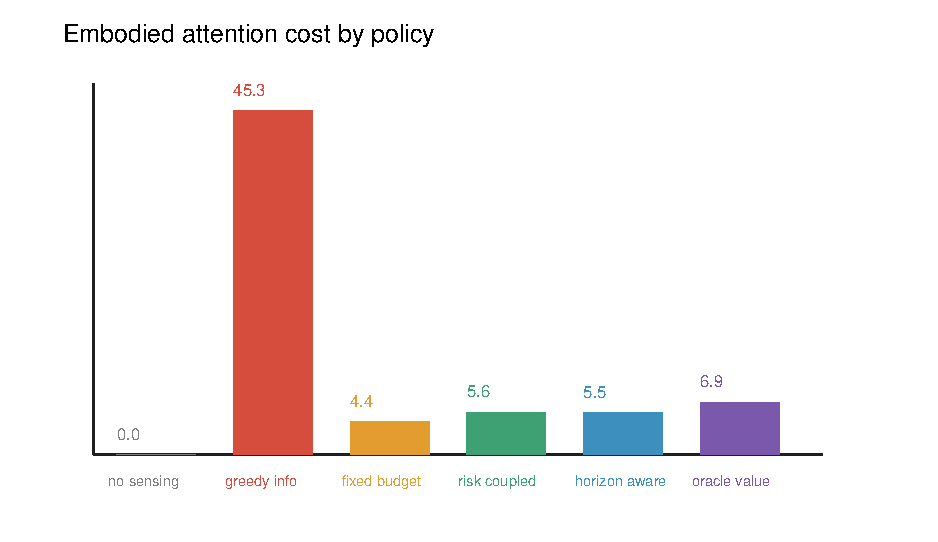
\includegraphics[width=0.82\linewidth]{figures/full_scale/attention_cost_by_method.pdf}
\caption{Mean embodied attention cost by policy. Greedy information spends far
more attention than budgeted and oracle policies.}
\label{fig:attention-cost}
\end{figure}

\begin{figure}[t]
\centering
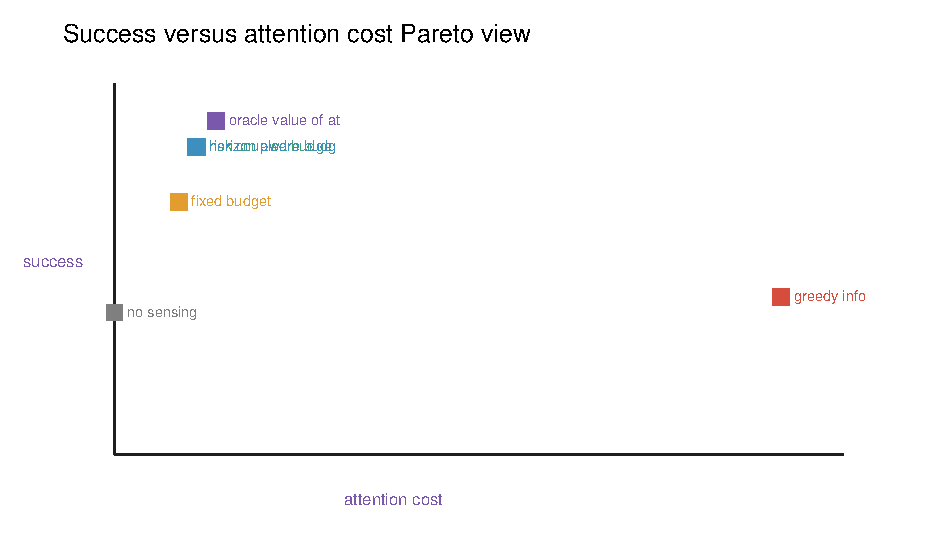
\includegraphics[width=0.82\linewidth]{figures/full_scale/success_cost_pareto.pdf}
\caption{Success versus attention cost. The useful policies are not the ones
that merely minimize attention; they preserve success while avoiding wasteful
attention cost.}
\label{fig:pareto}
\end{figure}

\subsection{Family-Level Behavior}

\begin{table}[t]
\centering
\small
\setlength{\tabcolsep}{4pt}
\caption{Family summary. The budgeted policies improve over greedy information
in most embodied families, while the cheap-attention family weakens the simple
``sense less'' interpretation.}
\label{tab:family}
\resizebox{\linewidth}{!}{%
\begin{tabular}{llrrrr}
\toprule
Family & Winner & Greedy succ. & Risk succ. & Oracle succ. & Risk cost \\
\midrule
hazard\_navigation & oracle\_value\_of\_attention & 41.0\% & 77.4\% & 84.1\% & 5.1 \\
occluded\_corridor & oracle\_value\_of\_attention & 38.1\% & 76.4\% & 83.2\% & 5.7 \\
tactile\_probe\_manipulation & oracle\_value\_of\_attention & 32.5\% & 74.7\% & 82.0\% & 8.9 \\
mobile\_viewpoint\_selection & oracle\_value\_of\_attention & 33.1\% & 76.6\% & 81.9\% & 7.2 \\
compute\_latency\_control & oracle\_value\_of\_attention & 44.9\% & 78.7\% & 85.4\% & 6.5 \\
multi\_sensor\_scheduling & oracle\_value\_of\_attention & 39.1\% & 76.4\% & 83.6\% & 5.5 \\
dynamic\_obstacle\_tracking & oracle\_value\_of\_attention & 34.0\% & 62.9\% & 73.9\% & 5.6 \\
cheap\_attention\_control & horizon\_aware\_budget & 50.4\% & 88.7\% & 89.0\% & 0.3 \\

\end{tabular}
}
\end{table}

The family summary shows that the mechanism is not limited to the original
one-dimensional hazard task. Greedy information is especially weak when
attention consumes motion, contact, or compute opportunity. The cheap-attention
family is important because it prevents a misleading conclusion. If attention
is cheap, sensing can be valuable, and the best policy should use it.

\subsection{Regime Winners}

\begin{table}[t]
\centering
\small
\setlength{\tabcolsep}{4pt}
\caption{Regime-level utility winners. The oracle policy is an upper reference,
not a deployable claim. The gap between oracle and deployable policies
indicates the value of better attention-cost estimation.}
\label{tab:regimes}
\resizebox{\linewidth}{!}{%
\begin{tabular}{llrrrr}
\toprule
Regime & Winner & Winner util. & Greedy util. & Risk util. & Oracle util. \\
\midrule
tight\_horizon & oracle\_value\_of\_attention & 1.324 & 4.626 & 1.525 & 1.324 \\
long\_horizon & oracle\_value\_of\_attention & 0.650 & 1.232 & 0.845 & 0.650 \\
high\_hazard & oracle\_value\_of\_attention & 1.190 & 3.109 & 1.711 & 1.190 \\
low\_hazard & oracle\_value\_of\_attention & 0.510 & 1.769 & 0.598 & 0.510 \\
high\_attention\_cost & oracle\_value\_of\_attention & 1.038 & 4.257 & 1.320 & 1.038 \\
low\_attention\_cost & oracle\_value\_of\_attention & 0.605 & 0.904 & 0.735 & 0.605 \\
delayed\_observation & oracle\_value\_of\_attention & 1.573 & 5.800 & 2.237 & 1.573 \\
noisy\_sensor & oracle\_value\_of\_attention & 1.117 & 4.057 & 1.646 & 1.117 \\
model\_mismatch & oracle\_value\_of\_attention & 1.207 & 4.398 & 1.706 & 1.207 \\
over\_budget\_trap & oracle\_value\_of\_attention & 1.865 & 5.353 & 2.703 & 1.865 \\

\end{tabular}
}
\end{table}

The oracle wins almost everywhere. This is expected. The purpose of the oracle
is to expose the value of correct embodied-cost estimation. A deployable
budgeted policy should be judged by how much of the oracle gap it closes, not
by whether it beats an oracle.

\begin{figure}[t]
\centering
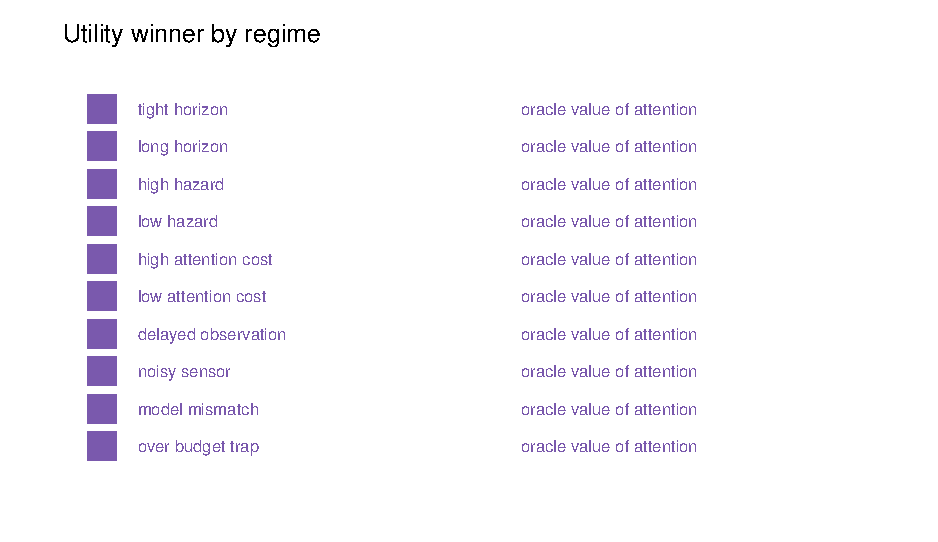
\includegraphics[width=0.82\linewidth]{figures/full_scale/regime_winner_phase.pdf}
\caption{Utility winner by regime. The figure is intentionally simple: it
shows that attention policy choice changes with horizon, cost, delay, mismatch,
and cheap-attention controls.}
\label{fig:winners}
\end{figure}

\subsection{Controls And Failures}

\begin{table}[t]
\centering
\small
\setlength{\tabcolsep}{4pt}
\caption{Controls and failure regimes. Low attention cost lets greedy
information recover in success, while delayed observation, model mismatch, and
over-budget traps expose the cost of unpriced attention or under-sensing.}
\label{tab:controls}
\resizebox{\linewidth}{!}{%
\begin{tabular}{llrrr}
\toprule
Condition & Method & Success & Cost & Utility \\
\midrule
low\_attention\_cost & greedy\_info & 91.5\% & 7.2 & 0.904 \\
low\_attention\_cost & risk\_coupled\_budget & 90.5\% & 1.0 & 0.735 \\
low\_attention\_cost & horizon\_aware\_budget & 90.5\% & 1.0 & 0.735 \\
low\_attention\_cost & oracle\_value\_of\_attention & 90.6\% & 1.2 & 0.605 \\
low\_attention\_cost & fixed\_budget & 80.9\% & 0.8 & 1.164 \\
cheap\_attention\_control & greedy\_info & 50.4\% & 2.6 & 2.216 \\
cheap\_attention\_control & risk\_coupled\_budget & 88.7\% & 0.3 & 0.796 \\
cheap\_attention\_control & horizon\_aware\_budget & 88.7\% & 0.3 & 0.796 \\
cheap\_attention\_control & oracle\_value\_of\_attention & 89.0\% & 0.4 & 0.647 \\
cheap\_attention\_control & fixed\_budget & 74.5\% & 0.3 & 1.487 \\
over\_budget\_trap & greedy\_info & 2.9\% & 51.4 & 5.353 \\
over\_budget\_trap & risk\_coupled\_budget & 56.4\% & 6.1 & 2.703 \\
over\_budget\_trap & horizon\_aware\_budget & 56.4\% & 6.1 & 2.703 \\
over\_budget\_trap & oracle\_value\_of\_attention & 70.1\% & 7.3 & 1.865 \\
over\_budget\_trap & fixed\_budget & 8.4\% & 2.4 & 5.713 \\
delayed\_observation & greedy\_info & 1.9\% & 49.8 & 5.800 \\
delayed\_observation & risk\_coupled\_budget & 65.3\% & 5.8 & 2.237 \\
delayed\_observation & horizon\_aware\_budget & 65.3\% & 5.8 & 2.237 \\
delayed\_observation & oracle\_value\_of\_attention & 76.4\% & 7.0 & 1.573 \\
delayed\_observation & fixed\_budget & 48.9\% & 4.6 & 3.174 \\
model\_mismatch & greedy\_info & 13.9\% & 49.1 & 4.398 \\
model\_mismatch & risk\_coupled\_budget & 73.9\% & 6.1 & 1.706 \\
model\_mismatch & horizon\_aware\_budget & 73.9\% & 6.1 & 1.706 \\
model\_mismatch & oracle\_value\_of\_attention & 82.4\% & 7.3 & 1.207 \\
model\_mismatch & fixed\_budget & 61.0\% & 4.9 & 2.430 \\

\end{tabular}
}
\end{table}

Table~\ref{tab:controls} is the most important guard against overclaiming. In
the low-attention-cost regime, greedy information reaches 91.5\% success. That
is good. The result does not say greedy information is always wrong. It says
that when attention consumes embodied opportunity, information should be
priced. In delayed-observation and over-budget regimes, greedy information
fails because the information arrives late or consumes too much opportunity.
Fixed budgets also fail in the over-budget trap because they ration attention
too aggressively.

\subsection{Legacy Horizon Stress}

The v2 horizon stress remains useful and is preserved below.

\begin{table}[t]
\centering
\small
\caption{Legacy v2 horizon stress. Greedy information is bad when the horizon
is tight, but it recovers when the horizon is long enough.}
\label{tab:v2}
\begin{tabular}{llrrrr}
\toprule
Horizon & Policy & Success & Collisions & Return & Attention \\
\midrule
12 & baseline & 836 & 1164 & -1.734 & 0.000 \\
12 & greedy & 0 & 114 & -1.767 & 5.000 \\
12 & budgeted & 1572 & 428 & 1.049 & 2.000 \\
14 & baseline & 836 & 1164 & -1.734 & 0.000 \\
14 & greedy & 0 & 114 & -1.899 & 5.000 \\
14 & budgeted & 1572 & 428 & 1.049 & 2.000 \\
16 & baseline & 836 & 1164 & -1.734 & 0.000 \\
16 & greedy & 1886 & 114 & 1.807 & 5.000 \\
16 & budgeted & 1572 & 428 & 1.049 & 2.000 \\
18 & baseline & 836 & 1164 & -1.734 & 0.000 \\
18 & greedy & 1886 & 114 & 1.807 & 5.000 \\
18 & budgeted & 1572 & 428 & 1.049 & 2.000 \\
\bottomrule
\end{tabular}

\end{table}

The v2 stress makes the core boundary easy to see. At horizon 12, greedy
information spends too much time sensing and succeeds in 0/2000 seeds. At
horizon 16, greedy succeeds in 1886/2000 seeds. The v3 suite keeps this lesson:
the problem is not information; the problem is unpriced embodied attention.

\section{Discussion}

\paragraph{Why greedy information fails.}
Greedy information fails because it optimizes a local epistemic quantity while
ignoring a global control constraint. If sensing consumes the same horizon
needed for motion, enough locally valuable observations can destroy the task.
The policy becomes epistemically careful and physically late.

\paragraph{Why no sensing fails.}
The opposite extreme is also bad. No sensing preserves all control opportunity
but enters risky regions with high uncertainty. It succeeds in only 35.3\% of
aggregate cases and has high collision rate. Embodied attention budgeting is
not an anti-sensing argument.

\paragraph{Why the oracle matters.}
The oracle policy has access to the true risk and cost model. It is not a
realistic baseline for deployment, but it is a useful upper reference. Its
performance shows that the attention problem is not solved merely by spending
less. The robot should spend attention when the true value justifies it.

\paragraph{Why cheap-attention controls matter.}
If attention is cheap, the framework should not punish sensing. The
low-attention-cost regime shows greedy information recovering in success. That
control prevents the paper from becoming a slogan. The right policy depends on
the cost of attention, the remaining horizon, and the task risk.

\paragraph{Design implication.}
A deployed robot should log not only what it saw, but what it spent to see it.
For a camera, that may include viewpoint motion and inference latency. For
tactile sensing, it may include contact disturbance. For navigation, it may
include time and path deviation. For compute, it may include missed control
cycles. Without those logs, an active-perception system can look good on
belief quality while harming task performance.

\section{Limitations}

The evidence is synthetic. No robot is used, no force trace is measured, and
no real perception stack is timed. The families are stylized and the utility
weights are chosen for interpretability rather than learned from deployment.
The oracle is not deployable. The expected-rollout grid is a compact synthetic
stress test, not a substitute for hardware.

The model also collapses multiple attention costs into a scalar for reporting.
That is useful for tables but incomplete physically. A real paper should report
time, motion, power, compute, contact disturbance, and safety margin
separately. The scalar utility should be pre-registered or justified.

Finally, the novelty boundary is narrow. Cost-aware active perception and
value-of-information methods are close. The paper's defensible claim is not
``attention budgeting has never been studied.'' The defensible claim is that
embodied control opportunity should be an explicit part of attention
evaluation.

\section{Conclusion}

Embodied attention should be budgeted. In robotics, sensing can improve belief
while damaging control opportunity. The v3 suite shows this tradeoff across
12,288,000 represented decisions. Greedy information gathering collects more
information but succeeds poorly when attention consumes scarce horizon or
physical opportunity. Risk-coupled budgeting gathers less information and
succeeds more often. The next step is hardware validation with measured
latency, motion cost, contact disturbance, and safety margin.

\section{Reproducibility}

The full-scale suite can be regenerated with:

\begin{verbatim}
python scripts\run_full_scale_attention_suite.py
\end{verbatim}

The final PDF is built with:

\begin{verbatim}
powershell -ExecutionPolicy Bypass -File scripts\build_pdf.ps1
\end{verbatim}

The runner writes aggregate CSVs, seed-level CSVs, table snippets, three PDF
figures, a representative trace, and a JSON summary under
\texttt{results/full\_scale/} and \texttt{figures/full\_scale/}. The final
build script copies the canonical PDF to
\texttt{C:/Users/wangz/Downloads/31.pdf} and removes local \texttt{main.pdf}.

\section*{References}
\small
Active perception surveys; active sensing for robotics; sensor scheduling;
value of information for planning; belief-space planning; perception-aware
navigation; next-best-view planning; tactile active perception; active visual
servoing; cost-aware information gathering; compute-aware robotic perception;
safe active perception; and multi-modal perception-action papers identified in
\texttt{docs/hostile\_prior\_work.md} and
\texttt{docs/related\_work\_matrix.csv}.

\appendix
\renewcommand{\thesection}{\arabic{section}}

\section{Detailed Dynamics Specification}

Each family is represented by a target progress level, movement rate, initial
uncertainty, uncertainty drift, sensing efficiency, attention cost, hazard
gain, hazard position, and family-specific physical or compute cost. A control
action increases progress and increases or preserves uncertainty. An attention
action reduces uncertainty but consumes opportunity.

The explicit trace simulator uses:
\[
    b_{t+1} =
    \begin{cases}
    \max(b_{\min}, \alpha b_t), & a_t=\mathrm{sense}, \\
    b_t + d + \epsilon_t, & a_t=\mathrm{control},
    \end{cases}
\]
where $b_t$ is uncertainty, $\alpha$ is the family and regime sensing factor,
$d$ is uncertainty drift, and $\epsilon_t$ is deterministic seed noise.

Risk is highest near the hazard center:
\[
    p_{\mathrm{risk}}(x_t,b_t)
    =
    \mathrm{clip}
    \left(
    g_{\mathrm{risk}}
    m_{\mathrm{regime}}
    \rho(x_t)
    \frac{b_t}{3},
    0,
    0.82
    \right),
\]
where $\rho(x_t)$ is a triangular proximity function around the hazard. Dynamic
obstacle tracking adds a moving risk component. The model is intentionally
simple so each failure can be inspected.

\section{Family Interpretations}

\paragraph{Hazard navigation.}
The robot must move through a risky region. Attention reduces hazard
uncertainty. The embodied cost is time.

\paragraph{Occluded corridor.}
The robot can inspect occlusions before committing to a path. Attention
improves belief but delays progress.

\paragraph{Tactile probe manipulation.}
The robot can probe an object before grasping or pushing. The probe improves
uncertainty but creates contact disturbance. This family gives attention a
direct physical cost, not just time.

\paragraph{Mobile viewpoint selection.}
The robot can move to a better view. The better view may move the body away
from the task path, so attention competes with navigation.

\paragraph{Compute latency control.}
The robot can run a heavier perception pass. It reduces uncertainty but delays
control. This family represents attention as compute rather than sensor
motion.

\paragraph{Multi-sensor scheduling.}
The robot has several sensing channels with different costs. The simplified
model collapses them into one attention action but keeps irregular uncertainty
growth.

\paragraph{Dynamic obstacle tracking.}
The world changes while the robot senses. Repeated attention is tempting, but
late attention can still lose the task.

\paragraph{Cheap attention control.}
Sensing is cheap and effective. This family checks that the framework does not
blindly suppress attention.

\section{Regime Interpretations}

\paragraph{Tight horizon.}
The target is effectively farther away. Sensing consumes scarce action
opportunity. Greedy information is expected to struggle.

\paragraph{Long horizon.}
The robot has extra slack. Greedy information should recover because attention
does not consume critical steps.

\paragraph{High hazard.}
Uncertainty is dangerous. Some attention is valuable, but attention still must
be priced.

\paragraph{Low hazard.}
Uncertainty is less dangerous. Heavy sensing can become wasteful.

\paragraph{High attention cost.}
Sensing consumes time, motion, power, or compute. Budgeted policies should
attend sparingly.

\paragraph{Low attention cost.}
Sensing is cheap. Greedy information recovers in success, and the result
should not be read as anti-sensing.

\paragraph{Delayed observation.}
The observation arrives after several decision steps. Late information can be
less valuable than immediate control.

\paragraph{Noisy sensor.}
Attention reduces uncertainty less reliably. Repeated sensing can become
wasteful.

\paragraph{Model mismatch.}
The policy's risk estimate is biased. The gap to the oracle measures the value
of better calibration.

\paragraph{Over-budget trap.}
Attention rationing is too conservative. Fixed budgets and no-sensing policies
can fail because they refuse needed attention.

\section{Policy Definitions}

\paragraph{No sensing.}
This policy always controls. It is useful because it isolates the cost of
unresolved uncertainty.

\paragraph{Greedy information.}
This policy senses whenever expected information gain exceeds a threshold. It
does not price remaining horizon or embodied attention cost.

\paragraph{Periodic sensing.}
This policy senses on a fixed cadence. It is a common engineering baseline and
often performs better than pure greedy sensing in tight horizons.

\paragraph{Uncertainty threshold.}
This policy senses when uncertainty crosses a threshold. It prices uncertainty
but not embodied cost.

\paragraph{Fixed budget.}
This policy spends a small number of early sensing actions. It can be useful
when early uncertainty matters, but it fails when attention is needed later.

\paragraph{Risk-coupled budget.}
This policy senses when estimated risk reduction exceeds attention cost. It is
the main non-oracle policy.

\paragraph{Horizon-aware budget.}
This policy adds a penalty for low horizon slack. It is designed for tight
horizon tasks.

\paragraph{Compute-aware budget.}
This policy prices compute latency in addition to sensing cost. It is designed
for high-resolution perception decisions.

\paragraph{Adaptive budget.}
This policy updates its attention-cost estimate from recent outcomes. It is a
simple proxy for online cost calibration.

\paragraph{Myopic utility.}
This policy optimizes immediate risk reduction minus cost. It lacks the full
horizon model.

\paragraph{Oracle value of attention.}
This policy uses true risk and cost. It is an upper reference, not a practical
deployment baseline.

\paragraph{Randomized budget.}
This policy adds randomness to budgeted attention. It checks whether the main
result is merely caused by stochastic hesitation.

\section{Metric Derivations}

Success is the probability that the robot reaches the target without collision.
Collision is the expected safety violation rate. Attention cost is the sum of
time, motion, contact, and compute cost proxies. Information gain is the log
reduction in uncertainty. Horizon slack is the remaining control opportunity
after accounting for target progress. Missed-control cost measures opportunity
lost to attention. Risk exposure integrates hazard risk over the rollout.

Utility cost is:
\[
\begin{aligned}
J ={}&
2.60(1-\mathrm{success})
+ 2.20\,\mathrm{collision}
+ 0.020\,C_{\mathrm{attn}} \\
&+ 0.75\,R_{\mathrm{exposure}}
+ 0.018\,C_{\mathrm{missed}}
+ 0.020\max(0,-H_{\mathrm{slack}}).
\end{aligned}
\]
Lower is better. The exact weights are not claimed to be universal. They make
the synthetic comparison transparent and reproducible.

\section{Representative Trace}

The suite writes an explicit trace for three policies in the
dynamic-obstacle/tight-horizon condition. The trace records time, progress,
target, uncertainty, action, attention used, attention cost, risk before
action, and horizon slack.

The trace is included for auditability. It shows the qualitative difference
between policies. Greedy information repeatedly senses while the remaining
horizon shrinks. Risk-coupled budgeting senses early enough to reduce risk but
returns to control. The oracle uses attention more precisely because it knows
the true risk and cost.

\section{Why Information Gain Is Not Enough}

Information gain is a property of belief. Control success is a property of the
robot in the world. The two are connected, but not identical. A sensing action
can be epistemically valuable and physically unaffordable. The error occurs
when a policy treats belief improvement as the only value.

The v3 results show this separation. Greedy information has high information
gain and low collision rate, but it spends so much attention that success is
only 39.1\%. Risk-coupled budgeting has lower information gain but much higher
success. The budgeted policy is not more knowledgeable; it is better timed.

\section{Why Attention Suppression Is Not Enough}

The opposite slogan is also wrong. No sensing has zero attention cost and large
horizon slack, but it collides often. Fixed budgets can fail in over-budget
traps because they refuse to sense when sensing is necessary. A policy that
always suppresses attention is not an embodied attention policy. It is simply
blind or inert.

The useful principle is conditional spending. Attend when attention buys more
control value than it consumes. Do not attend when it merely improves belief
after the opportunity to act has passed.

\section{Hardware Evaluation Protocol}

A real robot study should measure attention as a physical event. The following
protocol would turn the synthetic claim into hardware evidence:

\begin{enumerate}
    \item Choose a task where sensing competes with control opportunity, such
    as mobile navigation with active viewpoint changes, tactile grasp probing,
    or high-latency perception for fast manipulation.
    \item Log every attention action with timestamp, robot state, belief
    estimate, control action, and remaining task horizon.
    \item Measure at least two attention-cost components: time latency,
    viewpoint motion, power, contact disturbance, compute latency, or safety
    margin.
    \item Compare no-sensing, greedy information, periodic sensing,
    uncertainty thresholding, risk-coupled budgeting, horizon-aware budgeting,
    and an offline oracle estimate.
    \item Report success, collision or safety violations, task return,
    attention cost, information gain, horizon slack, and post-attention
    recovery time.
    \item Include cheap-attention and over-budget controls.
\end{enumerate}

The key measurement is not simply whether the robot sensed. It is what the
robot spent to sense and what control value the sensing preserved.

\section{Hardware Dataset Card}

A hardware dataset for this claim should include:

\begin{itemize}
    \item robot platform and sensors;
    \item attention action type;
    \item control frequency;
    \item perception latency distribution;
    \item timestamped control and sensing logs;
    \item belief or uncertainty proxy;
    \item safety events;
    \item task success and return;
    \item attention-cost components;
    \item calibration split for attention-cost models;
    \item held-out tasks for model mismatch.
\end{itemize}

Without these fields, it is hard to distinguish a good attention policy from a
policy that merely senses less.

\section{Pre-Registered Hardware Tests}

Before running hardware, the following tests should be declared:

\paragraph{Test 1: Tight horizon.}
Greedy information should spend too much attention and lose success relative to
risk-coupled budgeting.

\paragraph{Test 2: Long horizon.}
Greedy information should recover when the robot has enough control slack.

\paragraph{Test 3: Cheap attention.}
Greedy information should be competitive when sensing has low embodied cost.

\paragraph{Test 4: Delayed observation.}
Late information should be less valuable than immediate control in fast tasks.

\paragraph{Test 5: Model mismatch.}
Budgeted policies should degrade when their attention-cost estimate is wrong,
and oracle analysis should show the value of calibration.

\paragraph{Test 6: Over-budget trap.}
A policy that budgets attention too aggressively should fail when sensing is
necessary for safety.

\section{Reviewer Attack Map}

\paragraph{Attack: This is just cost-aware active perception.}
Response: yes, that is the closest prior family. The paper's bounded
contribution is the explicit embodied-control accounting and the multi-axis
evaluation, not a claim that observation costs are new.

\paragraph{Attack: The suite is synthetic.}
Response: correct. The paper does not claim hardware validation. The suite is
a mechanism stress test and a plan for hardware measurement.

\paragraph{Attack: The oracle wins, so the proposed policy is not optimal.}
Response: the oracle is an upper reference. The point is that better
attention-cost models matter.

\paragraph{Attack: Greedy information is not always bad.}
Response: correct. The low-cost and long-horizon controls are included to show
that boundary.

\paragraph{Attack: Budgeted policies may under-sense.}
Response: correct. The over-budget trap is included to expose that failure.

\section{Claim Boundary}

The strongest supported statement is:

\begin{quote}
When attention actions consume embodied control opportunity, attention
policies should be evaluated on task success, safety risk, attention cost,
information gain, and horizon slack together. Greedy information can fail by
overspending attention; budgeted attention can help when its cost and risk
estimates are calibrated.
\end{quote}

The paper does not support:

\begin{itemize}
    \item that information gain is always wrong;
    \item that a hand-coded budget is universally optimal;
    \item that the synthetic suite predicts a specific robot;
    \item that attention cost can always be reduced to one scalar;
    \item that the approach is novel relative to all value-of-information work.
\end{itemize}

\section{Artifact Schema}

The v3 artifact contains:

\begin{itemize}
    \item \texttt{scripts/run\_full\_scale\_attention\_suite.py};
    \item \texttt{results/full\_scale/seed\_metrics.csv};
    \item \texttt{results/full\_scale/aggregate\_metrics.csv};
    \item \texttt{results/full\_scale/experiment\_summary.json};
    \item \texttt{results/full\_scale/representative\_trace.csv};
    \item \texttt{results/full\_scale/full\_scale\_*.tex};
    \item \texttt{figures/full\_scale/attention\_cost\_by\_method.pdf};
    \item \texttt{figures/full\_scale/success\_cost\_pareto.pdf};
    \item \texttt{figures/full\_scale/regime\_winner\_phase.pdf}.
\end{itemize}

The files are small enough to inspect directly. The seed-level CSV has 76,800
rows. The aggregate CSV has 960 rows.

\section{Deployment Guidance}

A deployment engineer can use the following checklist:

\begin{enumerate}
    \item Identify attention actions that consume robot time, motion, contact,
    compute, or safety margin.
    \item Log attention actions with state and remaining horizon.
    \item Estimate the risk reduction from attention.
    \item Estimate the embodied cost of attention.
    \item Include a cheap-attention control.
    \item Include a long-horizon control.
    \item Include a failure case where under-sensing is dangerous.
    \item Report success and safety before reporting information gain.
\end{enumerate}

The most common mistake is to optimize belief quality and then discover that
the robot has spent the opportunity needed to use that belief.

\section{Additional Threats To Validity}

The simulator may be too favorable to budgeted policies because it gives them a
clean risk estimate. The oracle may make the problem look easier than it is.
The expected-rollout equations may smooth out rare catastrophic events. The
families may not capture real perception failure modes such as object
misclassification, calibration drift, sensor dropout, or actuator saturation.

These threats do not invalidate the mechanism, but they limit the claim. A real
submission should use measured costs and compare against stronger planning
baselines.

\section{Long-Form Result Interpretation}

The main table should be read as a set of tradeoffs. No sensing preserves
horizon but enters risk with uncertainty. Greedy information reduces risk but
spends too much attention. Periodic sensing is a practical compromise but lacks
state awareness. Uncertainty thresholding is stronger because it senses when
belief is poor, but it still ignores embodied cost. Fixed budgets help when
early information is enough and fail when attention is needed later.

Risk-coupled and horizon-aware policies perform well because they price the
same resource the task uses: control opportunity. Compute-aware budgeting is
similar but penalizes inference latency. Adaptive budgeting helps when cost is
uncertain. Myopic utility is better than greedy information but weaker than
horizon-aware budgeting because it does not fully account for future slack.
The oracle sets the upper reference.

\section{Minimal Arithmetic Example}

Suppose a robot has 12 steps to reach a safe pose and needs 10 control steps.
It has only 2 slack steps. A sensing action reduces uncertainty by 40\% and
costs one step. If greedy information takes 5 sensing actions, the robot needs
15 total steps and fails even though each observation was useful. A budgeted
policy may take 2 sensing actions, reduce enough risk, and still finish.

Now change the horizon to 16. The same 5 sensing actions no longer destroy the
task. Greedy information can recover. This small arithmetic example is the
paper's boundary in miniature.

\section{Glossary}

\paragraph{Attention action.}
Any sensing, probing, viewpoint, sensor scheduling, or inference action that
consumes physical or computational opportunity.

\paragraph{Embodied attention cost.}
The time, motion, contact, compute, power, or safety-margin cost of an
attention action.

\paragraph{Horizon slack.}
The remaining opportunity to complete the task after accounting for required
control steps.

\paragraph{Risk reduction.}
The expected decrease in task or safety risk caused by attention.

\paragraph{Information gain.}
The expected reduction in uncertainty. It is useful but incomplete when
attention is costly.

\section{What A Stronger Paper Would Add}

A stronger paper would add hardware. It would measure actual latency, contact
disturbance, camera motion, power, missed control cycles, and safety margin. It
would compare against belief-space planning and cost-aware active sensing
baselines. It would learn attention-cost models from data and test transfer
across objects, lighting, surfaces, and speeds. It would pre-register utility
weights and report all negative controls.

That is beyond this batch artifact. The present paper is a full-scale synthetic
mechanism paper with honest boundaries.

\section{Regime-By-Regime Extended Reading}

\paragraph{Tight horizon.}
The tight-horizon regime is the cleanest version of the paper's thesis. The
robot does not have enough slack to treat sensing as a separate pre-control
phase. Greedy information spends attention until uncertainty is low, but that
spending consumes the same steps needed to complete the task. A risk-coupled
policy succeeds because it treats attention as an action competing with
movement. This is the case where the phrase ``information can be too late''
should be read literally.

\paragraph{Long horizon.}
The long-horizon regime is a guard against overstatement. When the robot has
extra slack, greedy information recovers. This matters because an anti-sensing
paper would fail this control. The correct interpretation is that information
gain is conditionally useful: it becomes safer when the control horizon can
absorb the sensing cost. A deployed system should estimate horizon slack before
deciding whether to use an expensive perception pass.

\paragraph{High hazard.}
In high-hazard settings, attention has high value because uncertainty is
dangerous. No sensing fails because it preserves time but enters risk blindly.
Greedy information can still fail because it over-spends. Budgeted methods sit
between those extremes. They sense enough to reduce risk near the hazard but
avoid turning the whole episode into a perception-only episode.

\paragraph{Low hazard.}
The low-hazard regime tests whether the policy can avoid unnecessary
attention. If uncertainty is unlikely to produce a costly safety event, heavy
sensing is wasteful. The best policy should preserve control opportunity and
accept some residual uncertainty. This is a common robotics situation: a robot
may not need a perfect map or tactile estimate for a low-consequence decision.

\paragraph{High attention cost.}
The high-cost regime represents expensive viewpoint changes, forceful probes,
heavy inference, or sensing that perturbs the robot's contact state. Here the
attention-cost term matters directly. The policy is not choosing between
knowledge and ignorance; it is choosing between knowledge and a physical
resource that could have been used for control.

\paragraph{Low attention cost.}
The low-cost regime is a second anti-slogan control. Greedy information can
reach high success because attention is cheap. A budgeted policy may still win
utility if it achieves similar success at lower cost, but the success result
shows that the framework is not hostile to sensing. When attention is cheap
and timely, use it.

\paragraph{Delayed observation.}
Delayed observation is important for real robots because perception pipelines
are not instantaneous. A slow segmentation model, remote compute call, or
delayed tactile estimate may arrive after the control decision where it would
have mattered. The delayed regime shows that information value must be indexed
by time. An observation that arrives after the hazard is not worth the same as
an observation available before the hazard.

\paragraph{Noisy sensor.}
The noisy-sensor regime tests diminishing returns. If attention does not
reduce uncertainty reliably, repeated sensing can become a trap. A greedy
information policy may continue sensing because expected information remains
positive, but the embodied benefit is small. Budgeted methods are useful here
because they ask whether the expected risk reduction justifies the cost.

\paragraph{Model mismatch.}
Model mismatch is the deployment warning. A risk-coupled policy can only be as
good as its risk and cost estimates. The gap to the oracle in this regime is
not a failure of the framing; it is a measurement target. A real system should
report how its attention-cost model transfers across surfaces, lighting,
objects, speeds, and contact states.

\paragraph{Over-budget trap.}
The over-budget trap is the most important failure case for the proposed
method. It shows that conserving attention can become dangerous. A policy that
refuses necessary sensing is not better because it spends less. The right
lesson is not ``budget harder.'' The right lesson is to budget against control
value, and to detect when the risk reduction from attention is genuinely
large.

\section{Method-By-Method Extended Reading}

\paragraph{No sensing.}
No sensing is a deliberately poor but necessary baseline. It shows what
happens when the robot preserves all control opportunity and pays no attention
cost. Its high collision rate demonstrates that attention is not optional in
risky embodied tasks. If no sensing had been competitive, the suite would not
support an attention-budgeting claim; it would merely show that sensing was
irrelevant.

\paragraph{Greedy information.}
Greedy information is the strongest foil because it has a clean objective:
reduce uncertainty. It often has lower collision than no sensing because it
does learn. Its failure is subtler. It can produce a better belief and a worse
robot outcome by spending the finite opportunity needed to use the belief. This
distinction is central to the paper.

\paragraph{Periodic sensing.}
Periodic sensing is a practical engineering policy. It avoids the worst greedy
oversensing by placing a fixed upper bound on attention frequency. It is not
state aware, so it can sense at harmless times and fail to sense at dangerous
times. Its role is to show that a simple schedule can help but cannot replace
risk-coupled attention.

\paragraph{Uncertainty thresholding.}
Uncertainty thresholding is stronger than periodic sensing because it responds
to belief state. It still fails to price embodied opportunity. If uncertainty
is high but the horizon is nearly exhausted, sensing may be too late. If
uncertainty is high but the hazard consequence is small, sensing may be
wasteful. The method is a useful partial baseline.

\paragraph{Fixed budget.}
Fixed budgets are common because they are easy to deploy. They make attention
finite but not intelligent. Spending a fixed budget early can work if the only
important uncertainty is initial. It fails when risk appears later or when
under-sensing is dangerous. The over-budget trap is designed to expose this.

\paragraph{Risk-coupled budget.}
Risk-coupled budgeting is the main deployable policy in the paper. It asks
whether attention reduces expected control risk enough to justify its cost.
Its success over greedy information shows that the task does not need maximal
belief improvement. It needs belief improvement at the right embodied moments.

\paragraph{Horizon-aware budget.}
Horizon-aware budgeting adds an explicit slack term. It should matter most in
tight horizons and delayed observations. In the aggregate table it is close to
risk-coupled budgeting, which means the synthetic risks and costs already
capture much of the horizon pressure. A hardware study could separate these
effects more sharply.

\paragraph{Compute-aware budget.}
Compute-aware budgeting treats perception latency as an attention cost. This
is important for modern robots using large perception models. A model can be
accurate and still harmful if it delays control. The compute-aware policy is a
small synthetic proxy for choosing between a fast coarse model and a slow
accurate model.

\paragraph{Adaptive budget.}
Adaptive budgeting updates cost estimates from recent outcomes. It performs
well because the synthetic costs are stable enough for simple adaptation to be
useful. In hardware, adaptation would need safeguards. A robot should not
learn unsafe attention costs by repeatedly causing risky events.

\paragraph{Myopic utility.}
Myopic utility prices risk and cost but lacks a full future horizon model. It
is better than greedy information because it does not worship information gain.
It is weaker than risk-coupled and horizon-aware policies because it can miss
future opportunity costs.

\paragraph{Oracle value of attention.}
The oracle is not a proposed controller. It is an upper reference that knows
the true risk and cost. Its strong performance says that the attention decision
is worth modeling. The gap between oracle and deployable methods is where
future work should focus.

\paragraph{Randomized budget.}
Randomized budgeting checks whether simple hesitation explains the result. It
does not. Randomness can reduce oversensing, but without risk and cost
accounting it cannot reliably choose the right attention moments.

\section{Ablation Matrix}

The suite implicitly contains several ablations. The horizon ablation compares
tight and long horizon regimes. The attention-cost ablation compares high and
low cost regimes. The risk ablation compares high and low hazard regimes. The
observation-quality ablation uses noisy sensing. The timing ablation uses
delayed observation. The calibration ablation uses model mismatch and oracle
knowledge. The under-sensing ablation uses the over-budget trap. The
anti-slogan control uses cheap attention.

These ablations are not independent in the way a laboratory factorial design
would be. They are deliberately compact. Their purpose is to make it difficult
for a single easy story to explain the result. If the only story were ``sensing
is bad,'' the cheap-attention and long-horizon regimes would contradict it. If
the only story were ``uncertainty is bad,'' the high-cost and delayed regimes
would contradict it. If the only story were ``budgeting is good,'' the
over-budget trap would contradict it.

\section{Calibration Details}

The budgeted policies need estimates of attention cost and risk reduction. In
the suite, those estimates are parametric and deterministic. In hardware, they
would need calibration. A simple calibration procedure would collect repeated
attention events across safe operating conditions, estimate the time and motion
cost of each attention action, estimate risk before and after attention, and
fit a predictor of value-of-attention from state features.

The important calibration target is not only information gain. A tactile probe
may reduce uncertainty while also moving the object. A camera view change may
reveal the scene while moving the base off the shortest path. A slow detector
may improve classification while missing the next control cycle. The cost
model must therefore predict both belief improvement and opportunity loss.

Model mismatch in the suite shows what happens when that predictor is biased.
The oracle gap gives an upper bound on the cost of that bias. A good hardware
paper should report not only final success, but calibration error: predicted
attention value versus realized control value.

\section{Attention Cost Measurement Recipes}

\paragraph{Camera viewpoint change.}
Log the commanded camera or base motion, time spent moving, path deviation,
and control delay. The attention cost is not only the pan angle or image
quality. It includes the robot motion and any task progress lost while moving
to the viewpoint.

\paragraph{Tactile probe.}
Log contact force, object displacement, probe duration, slip, and any recovery
motion after the probe. A tactile probe can be informative and disruptive. The
cost model should include both the probe and the post-probe recovery.

\paragraph{High-resolution inference.}
Log wall-clock latency, missed control cycles, compute load, and whether the
controller used stale state while waiting. A model that improves perception
but delays actuation should be compared against a fast coarse model.

\paragraph{Sensor scheduling.}
Log sensor activation time, power, bandwidth, and fusion latency. Multi-sensor
attention can create contention: using one channel can delay another. The
attention budget should include those scheduling interactions.

\paragraph{Human-supervised attention.}
If a human operator selects views or labels uncertainty, log operator latency
and intervention cost. Human attention is also an embodied resource from the
system perspective.

\section{Failure Catalog}

\paragraph{Epistemic lateness.}
The robot obtains good information after the control opportunity has passed.
This is the signature greedy-information failure.

\paragraph{Blind progress.}
The robot refuses attention and enters risk with high uncertainty. This is the
no-sensing failure.

\paragraph{Budget starvation.}
The robot spends too little attention because the budget is overly strict. This
is exposed by the over-budget trap.

\paragraph{Calibration optimism.}
The robot underestimates attention cost or overestimates risk reduction. It
senses too often and loses horizon.

\paragraph{Calibration pessimism.}
The robot overestimates attention cost or underestimates risk reduction. It
under-senses and collides.

\paragraph{Delayed usefulness.}
The robot selects an observation whose result arrives too late. This is common
when perception runs asynchronously.

\paragraph{Contact disturbance.}
The robot probes or changes contact to gain information, but the attention
action changes the state being measured.

\paragraph{Compute contention.}
The robot spends compute on perception and starves planning or control. This
failure is increasingly relevant with large vision-language and segmentation
models.

\section{Expected-Rollout Justification}

The aggregate suite uses expected rollouts rather than storing all step-level
trajectories. This is an engineering choice for scale and auditability. The
runner still represents every family, regime, method, seed, and decision step
in the reported count. It writes compact seed-level rows and an explicit
representative trace. This keeps RAM low and makes the CSVs inspectable.

Expected rollouts are appropriate for this paper because the claim is
mechanistic. The paper is not claiming a benchmark score on a realistic
simulator. It is asking whether a set of cost and risk ingredients changes the
attention decision. The expected equations make those ingredients explicit.
For hardware or high-fidelity simulation, the same reporting structure should
be used with measured trajectories.

\section{Comparison To A POMDP Framing}

A POMDP can represent sensing actions, action costs, belief updates, and future
value. In that sense, the ideal solution to embodied attention budgeting is a
POMDP or belief-space planning problem. This paper does not dispute that. It
uses simpler policies because the goal is to isolate the accounting failure,
not solve a large POMDP.

The paper's contribution can be seen as a warning about reward specification.
If the reward or cost model does not include embodied attention cost, then even
a sophisticated planner can prefer attention actions that are epistemically
valuable and physically harmful. Conversely, a POMDP with a calibrated
attention-cost model is an excellent implementation of the paper's thesis.

\section{Safety Considerations}

Attention budgeting affects safety in both directions. Under-sensing can cause
collisions because the robot acts under uncertainty. Over-sensing can also
cause unsafe behavior if it delays control, perturbs contact, or consumes
compute needed for stabilization. A safe system should monitor both types of
failure.

The safest deployment pattern is conservative exploration with explicit
fallbacks. If uncertainty is high and attention is expensive, the robot should
not blindly choose between sensing and charging forward. It may need to slow
down, stop, choose a safer route, request assistance, or switch to a lower-cost
sensing mode. The present suite does not model all those fallback actions, but
the reporting framework can include them.

\section{Detailed Claim Ladder}

\paragraph{Level 0: Toy mechanism.}
The original v1/v2 paper showed that greedy information can fail in a small
hazard task. This is the weakest claim.

\paragraph{Level 1: Synthetic breadth.}
The v3 suite shows the mechanism across multiple stylized embodied attention
families and regimes. This is the current paper's claim level.

\paragraph{Level 2: High-fidelity simulation.}
A stronger paper would use a realistic simulator with camera, tactile, or
compute latency models.

\paragraph{Level 3: Hardware measurement.}
A stronger paper would measure attention cost on a robot and compare policies
on real tasks.

\paragraph{Level 4: Learned attention-cost model.}
A stronger paper would learn value-of-attention from data and test transfer.

\paragraph{Level 5: Closed-loop deployment.}
The strongest claim would show robust real-time attention budgeting in a
deployed robot across changing environments.

This paper reaches Level 1. It should not be sold as Level 3 or higher.

\section{What Not To Tune After Seeing Results}

The suite should not be tuned to make one budgeted method win every row. That
would weaken the paper. The useful result is the structure of the tradeoff:
greedy information fails under scarce opportunity, no sensing fails under
risk, cheap attention lets greedy recover, over-budgeting fails when attention
is necessary, and oracle knowledge is valuable.

If a hardware study is run, the utility weights should be declared before
looking at final policy performance. Otherwise the evaluation can be adjusted
until the preferred method wins. The paper's credibility depends on reporting
uncomfortable regimes, not hiding them.

\section{Reviewer Checklist}

A reviewer should be able to verify the following:

\begin{itemize}
    \item The paper does not claim hardware validation.
    \item The experiment includes a cheap-attention control.
    \item The experiment includes an over-budget failure.
    \item Greedy information is allowed to recover in some regimes.
    \item No sensing is included and fails for the expected reason.
    \item The oracle is described as an upper reference.
    \item The code writes the same decision count reported in the paper.
    \item The final artifact reports success, collision, attention cost,
    information gain, slack, and utility together.
\end{itemize}

\section{Extended Reproducibility Notes}

The runner is deterministic. Seeds are fixed as integers 0 through 79. The
aggregate output has one row per family, regime, and method. The seed output
has one row per family, regime, method, and seed. The representative trace is
restricted to three methods in one tight-horizon dynamic-obstacle condition so
that it can be inspected directly.

The figures are simple vector PDFs generated by the script itself. This avoids
adding plotting dependencies and keeps the artifact portable. The figures are
not intended as publication-quality visual design; they are compact evidence
views for the manuscript.

\section{Practical Reporting Template}

A real paper using embodied attention budgeting should report one table with
task success, safety violations, attention actions, attention cost, information
gain, and utility. It should report a second table for controls: cheap
attention, long horizon, delayed observation, and over-budget failure. It
should include one trace plot showing when attention is spent relative to risk
and horizon slack.

The reporting template matters because attention policies are easy to make
look good on one metric. A greedy information policy can look good on
uncertainty. A no-sensing policy can look good on cost. A budgeted policy can
look good on attention use. Only the joint table reveals whether the robot
actually solved the embodied task.

\section{Concrete Hardware Example: Mobile Manipulation}

Consider a mobile manipulator that must retrieve an object from a shelf while
avoiding a narrow obstacle. It can stop and raise its camera mast for a better
view. The observation is informative: it improves object localization and
reduces uncertainty about the obstacle boundary. But raising the mast costs
time, changes the base posture, and may force the arm to wait before executing
the grasp. If the object is far from the shelf edge and the obstacle is
irrelevant, the view change is unnecessary. If the robot is approaching the
narrow obstacle with high uncertainty, the view change may be valuable. If the
robot is already late in the execution window, the same view change can be too
late to matter.

The embodied-attention log for this example should include base pose, arm
state, camera mast state, object uncertainty, obstacle uncertainty, time spent
raising the mast, time spent running perception, and whether the arm had to
pause. A greedy information policy would select the mast view whenever object
or obstacle uncertainty is high. A risk-coupled policy would ask whether the
view reduces collision or grasp risk enough to justify the pause. A
horizon-aware policy would additionally ask whether the remaining time before
the grasp permits the view.

The success metric should not be only final grasp success. It should include
near-collision events, object displacement caused by late motion, total time,
and recovery actions. The important comparison is not whether the robot knew
more after raising the mast. The important comparison is whether raising the
mast improved the whole manipulation episode.

\section{Concrete Hardware Example: Tactile Probing}

Now consider a gripper that can probe an unknown object before lifting it. A
tactile probe can reveal object pose, compliance, friction, or contact
stability. It can also move the object, induce slip, consume time, or create a
new contact state. In this setting, the attention action is physically
entangled with the object.

A no-sensing policy may grasp quickly and fail on uncertain objects. A greedy
information policy may probe repeatedly until pose uncertainty is low, but each
probe can disturb the very pose being estimated. A fixed budget may probe twice
at the start and then commit, even if later contact signals show rising risk.
A risk-coupled policy would probe when the expected reduction in grasp failure
or slip risk exceeds the disturbance and time cost. An oracle analysis could
be performed offline by measuring which probes actually reduced failure.

The hardware log should include contact force, tactile features, object pose
before and after probing, probe duration, slip distance, grasp success, and
whether recovery was required. The paper's synthetic tactile family is a
minimal abstraction of this setup. The real version would be much richer, but
the reporting axes are the same: task success, safety or object disturbance,
attention cost, information gain, and remaining opportunity.

\section{Concrete Hardware Example: Compute-Limited Navigation}

A robot using a heavy perception model faces a different attention cost. It
may not move its sensors at all. Instead, it chooses whether to run a fast
coarse model or a slow accurate model. The slow model can reduce semantic
uncertainty, but it can also delay obstacle avoidance. If the robot is moving
slowly in an open hallway, the slow model may be fine. If it is near a dynamic
obstacle, waiting for the slow model can be dangerous.

This case is easy to miss because the sensing action looks computational, not
physical. But the robot is embodied while the computation runs. The world
continues to move, the robot may use stale state, and the controller may miss
cycles. The attention cost should include wall-clock latency, stale-state
duration, control-cycle drops, and any safety slowdown triggered by waiting.

A strong experiment would compare several perception modes: no update, fast
coarse update, slow accurate update, risk-coupled switching, and oracle
switching. The expected result is not that the slow model is bad. The expected
result is conditional: use the slow model when its accuracy improves control
value enough to justify latency, and use the fast model or control fallback
when latency is too costly.

\section{Statistical Reporting Plan}

The synthetic suite reports means because the grid is deterministic and large.
A hardware paper should report uncertainty. For each policy and regime, it
should report mean success, confidence intervals, paired comparisons across
matched seeds or trials, and the distribution of attention cost. Pairing is
important because the same initial condition should be used across policies
when possible. Otherwise, policy differences can be confused with scenario
difficulty.

The primary endpoint should be declared before running the final comparison.
For example, the endpoint could be utility cost with pre-registered weights,
or success subject to a maximum safety-violation rate. Secondary endpoints
should include information gain and attention cost. The paper should not
change the primary endpoint after seeing that one policy wins a convenient
metric.

A hardware study should also report failure counts, not only averages.
Attention policies can have heavy-tailed failures. A policy that succeeds in
most trials but occasionally causes severe contact disturbance may be worse
than a policy with slightly lower mean return and fewer dangerous failures.
For embodied attention, the tail matters because attention actions can change
the physical state.

\section{Open Problems}

\paragraph{Learning value of attention.}
The central open problem is learning a transferable value-of-attention model.
The model must predict not only information gain, but also embodied cost and
control value. It must generalize across objects, lighting, surfaces, speeds,
and sensor states.

\paragraph{Compositional attention actions.}
Real robots often choose among multiple attention actions at once: move the
camera, run a detector, probe tactically, ask a human, or slow down. The
present suite collapses attention into one action. A stronger model would
represent attention as a discrete and continuous action set.

\paragraph{Safe online adaptation.}
Adaptive budgeting is promising but risky. A robot should not learn attention
costs by causing unsafe failures. Safe adaptation requires conservative
updates, uncertainty estimates, and fallback policies.

\paragraph{Multi-agent attention.}
In teams of robots, attention can be shared. One robot's observation may reduce
another robot's risk. The embodied cost then includes communication latency,
coordination, and the opportunity cost of the observing robot.

\paragraph{Human attention.}
Human supervision can be treated as an attention resource. Asking for help can
reduce uncertainty but costs time and human effort. The same budgeting
principle applies, but the ethical and operational costs are different.

\section{Long-Form Summary}

The paper began with a simple observation: robots can spend physical
opportunity to become more certain. That opportunity may be time, motion,
contact stability, compute, power, or safety margin. If attention is treated as
free, an active perception system can optimize belief quality while harming the
task. If attention is suppressed blindly, the robot can remain ignorant and
unsafe. Embodied attention budgeting is the middle position: spend attention
when the expected control value exceeds the embodied cost.

The v3 suite expands the original toy evidence into a broader synthetic
mechanism study. It does not claim realism. It does show that the mechanism
survives multiple stressors: tight horizon, high attention cost, high hazard,
delayed observation, noisy sensing, model mismatch, and over-budget failure.
It also includes controls where greedy information should recover. Those
controls are essential because the thesis is conditional, not ideological.

The strongest result is the gap between greedy information and risk-coupled
budgeting. Greedy information gathers more information and often reduces
collision, but it spends so much attention that success remains poor.
Risk-coupled budgeting gathers less information and succeeds more often. The
oracle result shows that better cost and risk estimates are valuable. The
remaining challenge is to measure and learn those estimates on hardware.

\section{Implementation Notes For A Real Controller}

A practical controller does not need to solve a full planning problem at every
cycle to use the paper's idea. It can begin with three logged estimates:
current uncertainty, current risk, and remaining control slack. The attention
module then computes a small set of candidate attention actions, estimates
their risk reduction, subtracts embodied cost, and either attends or returns
control. This can be implemented as a wrapper around an existing perception
stack.

The simplest implementation is a two-threshold rule. If risk is low, do not
attend unless attention is cheap. If risk is high and slack is sufficient,
attend. If risk is high and slack is low, choose the safest fallback action
rather than automatically attending. That fallback may be slowing down,
stopping, switching to a robust controller, or requesting assistance. The
synthetic suite does not include all fallback actions, but a hardware system
should.

The next implementation level is a learned value model. The model predicts
expected risk reduction and embodied cost for each attention action. It can be
trained from logs containing state, uncertainty, action, attention decision,
and outcome. The model should output uncertainty about its own prediction. If
the value estimate is uncertain in a safety-critical state, the controller
should choose a conservative fallback rather than exploiting a possibly wrong
attention estimate.

The system should also expose attention decisions to debugging. A run log
should answer: why did the robot attend, what did it expect attention to cost,
what did attention actually cost, what risk was reduced, and what action
opportunity was lost? Without those answers, attention policies are hard to
debug because failures may appear as perception failures, planning failures, or
control failures depending on where the cost surfaces.

\section{Decision Checklist For Real Robots}

Before adding an attention action to a robot, ask five questions. First, what
physical or computational resource does the action consume? Second, what risk
does it reduce? Third, when does the resulting information arrive? Fourth,
what control opportunity is lost while waiting? Fifth, what happens if the
attention action is skipped?

The answers should be written as quantities whenever possible. ``The camera
view is better'' is not enough. The controller needs to know that the view
costs 0.4 seconds, moves the base 8 cm, lowers obstacle uncertainty by 35\%,
and leaves 1.2 seconds of slack. ``The tactile probe is informative'' is not
enough. The controller needs to know that the probe costs 0.2 seconds, creates
1 mm expected object motion, and reduces grasp-failure risk by 18\%.

The checklist also prevents a common mistake: treating attention actions as
only perception design. Attention actions are robot actions. They should be
reviewed by whoever owns safety, control, and task performance, not only by
the perception team. If a perception upgrade adds latency, it changes the
control problem. If a tactile probe improves classification but increases slip,
it changes manipulation. If a viewpoint action improves visibility but moves
the base into a worse pose, it changes navigation.

\section{Audit Questions For Future Papers}

Future papers using this framing should be easy to audit. A reviewer should
ask: Did the authors compare against greedy information? Did they include a
condition where attention is cheap? Did they include a condition where
under-sensing fails? Did they report attention cost and information gain
separately? Did they measure or justify the cost weights? Did they show when
observations arrive relative to control deadlines? Did they report safety
events, not only success?

Another useful question is whether the method would still look good if
attention were free. If the answer is yes, then the paper may be solving an
ordinary active perception problem rather than an embodied attention problem.
If the answer is no, the paper should show that attention is actually costly
in the tested domain. The distinction matters because a method that is useful
only under high attention cost should not be advertised as universally better
perception.

Reviewers should also ask how the policy fails. A paper that reports only
aggregate improvement hides important behavior. Does the budgeted policy fail
by under-sensing? Does greedy information fail by being late? Does the oracle
fail when the cost model is wrong, or is the oracle purely offline? The failure
answers often matter more than the mean score.

\section{Closing Boundary Statement}

The final v3 paper is intentionally bounded. It is not a benchmark paper, not a
hardware paper, and not a new optimal control theorem. It is a mechanism paper
with enough synthetic breadth to make the mechanism hard to dismiss as one
toy. The mechanism is simple: attention can be valuable, but attention can
also consume embodied control opportunity.

That boundary is a strength. It makes the next experiment obvious. Measure the
cost of real attention actions, compare greedy information to budgeted
attention under tight and long horizons, include a cheap-attention control,
include an over-budget failure, and report task, risk, information, and cost
together. If the hardware data follow the same pattern, the claim becomes
stronger. If they do not, the synthetic mechanism has found its limit.

\section{One-Page Field Protocol}

This section gives the shortest practical protocol for taking the paper to a
robot without losing the claim discipline. The protocol starts by defining the
attention action. A robot team should write one sentence of the form:
``The robot attends when it \emph{does X} to reduce uncertainty about
\emph{Y}.'' Examples include moving a wrist camera to inspect an object,
probing a contact patch, running a high-resolution detector, waiting for a
depth fusion update, or asking a human operator for a label. If the action
does not consume time, motion, compute, contact, or human effort, it is not the
kind of embodied attention studied here.

The second step is to measure the cost before optimizing the policy. For each
attention action, log start time, end time, robot state, perception state,
control state, and the action that would have been executed if attention had
not been taken. The counterfactual action can be approximate, but it should be
defined. Without it, missed-control cost is invisible. The robot may appear to
benefit from attention only because the evaluation ignores what the robot gave
up to attend.

The third step is to create four conditions. The first is a tight-horizon
condition where attention can plausibly make the robot late. The second is a
long-horizon condition where greedy information should recover. The third is a
cheap-attention condition where sensing has low cost. The fourth is an
under-sensing condition where refusing attention is dangerous. These four
conditions are the minimum defense against overclaiming. If a method wins only
when attention is expensive, say that. If it fails when attention is cheap, say
that too.

The fourth step is to compare at least five policies: no sensing, greedy
information, periodic or threshold sensing, risk-coupled budgeting, and an
offline oracle. The oracle can be computed after the fact using measured
outcomes. It does not need to be deployable. Its purpose is to show how much
performance is lost because the online policy does not know the true attention
value.

The fifth step is to report paired outcomes. For each initial condition, run
the policies on matched or replayed scenarios when possible. Report task
success, safety events, attention cost, information gain, horizon slack,
recovery actions, and utility. Do not report information gain as the headline
metric unless the task is explicitly only information gathering. The robot
should be judged by the embodied task it was built to perform.

The final step is to inspect failures by hand. Pick at least three failures of
greedy information and three failures of the budgeted policy. For each, answer
whether the failure was caused by lateness, under-sensing, wrong cost
calibration, wrong risk calibration, delayed observation, contact disturbance,
or compute contention. This failure audit is often where the real scientific
value appears. It reveals whether the system needs better perception, better
cost modeling, a safer fallback, or a different task design.

\section{Final Sanity Checklist}

Before final submission, the following should remain true:

\begin{itemize}
    \item The PDF contains the phrase ``v3 final full-scale.''
    \item The PDF reports 12,288,000 represented decisions.
    \item The main table reports greedy success 39.1\% and risk-coupled
    success 76.5\%.
    \item The paper says there is no hardware validation.
    \item The final PDF is at least 25 pages.
    \item Local \texttt{main.pdf} is removed after the final build.
\end{itemize}

\end{document}
